\DiaryEntry{Birthday Problem}{2022-12-16}{Stochastic}

The Birthday Problem considers a group of $N$ people and asks for the probability that more than $2$ share their birthday. This includes many cases: Two or more people sharing the same date and all others having different dates, but also two people sharing one date and three other people sharing another date etc.

Surprisingly, this probability becomes $\approx 50\%$ for $N = 23$ people and goes to almost $100\%$ for $N > 60$ people.

\paragraph{Proof.} We calculate the probability that \emph{no persons} share a birthday, $P(A')$. The event that all $N$ people have different birthdays is the same as the event that person $2$ does not have the same birthday as person $1$, that person $3$ does not have the same birthday as either person $1$ or person $2$, and so on, and finally that person $N$ does not have the same birthday as any of persons $1$ through $N-1$.

The probability that person $2$ does not have the same birthday as person $1$ is $\frac{364}{365}$, the probability that person $3$ does not have the same birthday as either person $1$ or person $2$ is $\frac{363}{365}$ and so on. Combining this, we arrive at

\bee
P(A') = \frac{364}{365} \times \frac{363}{365} \times \cdots \times \frac{365-N+1}{365} 
\eee

and from this we obtain for the probability that at least two persons share their birthday as

\bee
P_{bp} = 1 - \frac{364}{365} \times \frac{363}{365} \times \cdots \times \frac{365-N+1}{365} 
\eee

For $N=23$, we have $P_{bp} = 0.5073$ and for $N=50$ we have reached a probability of $97\%$. The "surprising" reason for the result is that we do \emph{not} consider the case where another person has the person as \emph{myself} (this would indeed be much lower) but we consider the case that \emph{any} two (or more) people share their birthday. And there are many more cases (e.g. person $5$ sharing with person $34$).

The following plot shows the probability as function of $N$.

\begin{figure}[H]
    \centering
    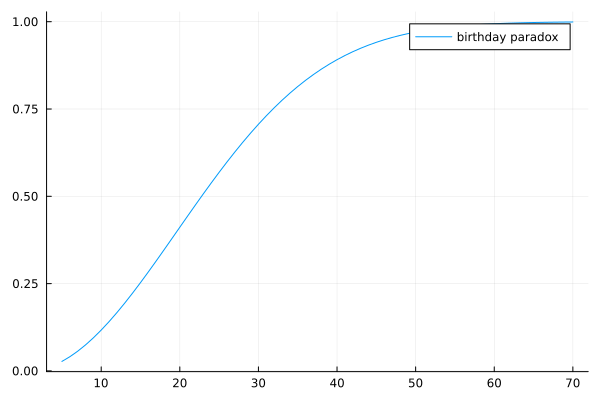
\includegraphics[scale=0.5]{images/2022-12-15-birthday_00.png}
\end{figure}


\paragraph{Extension / Explaination.} In the following, we consider a slightly more general setting (not restricted to a year) and use the following notation: Let $N$ denote the number of people and each is assigned a number drawn uniformly from the interval $[1,M]$.

Let's start by calculating the probability that exactely two persons draw the same number; the numbers assigned to the other $N-2$ persons are all different. We can chose two persons out of $N$ in ${N \choose 2}$ different ways and this pair is assigned one number out of $M$. The first person of the remaining $N-2$ gets a number from $M-1$ different values, the second person gets a number from $M-2$ different values and so on. We therefore have for the probability

\bee
P_2 = \left( {N \choose 2} 365 \times 364 \times 363 \times \cdots \times M-N+2 \right) \frac{1}{M^N}
\eee

where we have used the fact that assigning a number in $[1,M]$ to $N$ people can be done in $M^N$ different ways.

The following Figure shows the probability $P_2$ as function of $N$ for $M=365$

\begin{figure}[H]
    \centering
    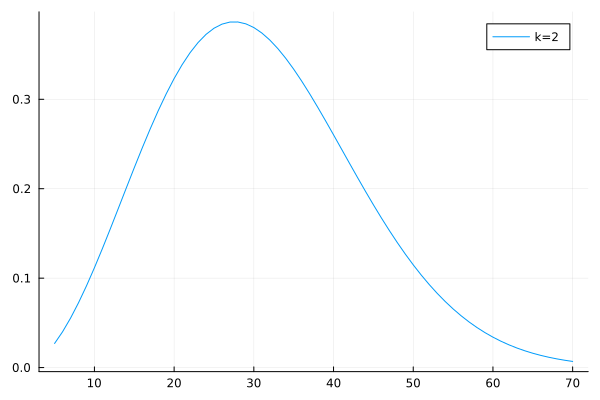
\includegraphics[scale=0.5]{images/2022-12-15-birthday_01.png}
\end{figure}

$P_2$ has a peak around $N \approx 28$ and falls off below and above this value. For values of $N < 28$, there are not enough people to share a birthday and therefore $P_2$ is small. The reason why $P_2$ is falling off for $N > 28$ is more interesting and will be pursued in the following.

The second interesting question is why $P_{bp} \rightarrow 1$ for large $N$ whereas $P_2 \rightarrow 0$ for large $0$. In other words, where does the probability come from?

As stated in the introduction, $P_{bp}$ includes also cases where three more people share the same number (and all others having different dates) and also cases, where two people share one date and three other people sharing another date. The "missing probability" must therefore come from these cases.

Let's start calculating the proability that two persons share a number, another two share another number, and the remaining $N-4$ people have all different numbers. We will denote this probability as $P_{2,2}$.

For the first duplicate, there are ${N \choose 2}$ ways to do this and we assign in a value in $[1,M]$. For the second duplicate, there are ${N-2 \choose 2}$ possibilities and we assign a value in $[1, M-1]$. For person $N-4$ we choose a value in $[1, M-2]$, for person $N-5$ we choose a value in $[1, M-3]$ and so on. For the last person we chose a value in $[1, M-N+5]$. 

We can exchange the positions of the two duplicates so we need to divide by $2! = 2$ and obtain

\bee
P_{2,2} = \frac{1}{2!} {N \choose 2} M {N-2 \choose 2} (M-1) \times (M-2) \times (M-3) \times \cdots \times (M-N+5) \frac{1}{M^N}
\eee

In a similar spirit, we obtain for the probability $P_{2,3}$ of three duplicates the following expression,

\bee
P_{2,3} = \frac{1}{3!}  {N \choose 2} M {N-2 \choose 2} (M-1) {N-4 \choose 2} (M-2) \times (M-3)\times \cdots \times (M-N+4) \frac{1}{M^N}
\eee

We have the following results for $M=365, N=50$: The probability for one duplicate is $P_2 \approx 0.115$, for two duplicates is $P_{2,2} \approx 0.20$, for three duplicates $P_{2,3} \approx 0.22$, and for four duplicates is $P_{2,4} \approx 0.16$. In other words, if there is ``enough space'' ($N$ is large), the probability of having more than one duplicate becomes larger.

The following plot shows the probability for different values of $N$.

\begin{figure}[H]
    \centering
    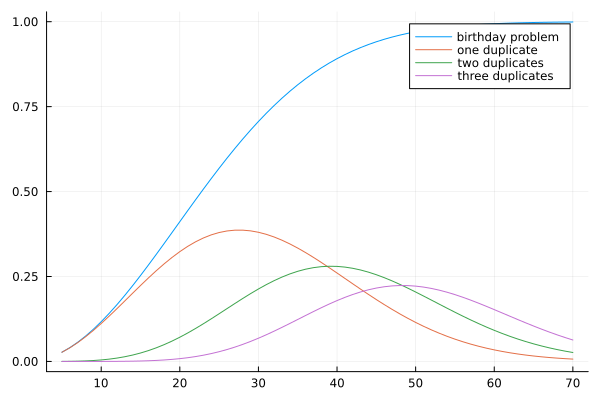
\includegraphics[scale=0.5]{images/2022-12-15-birthday_02.png}
\end{figure}

On the other hand, the probability $P_{k}$ of having $k$ persons sharing the same number is given by

\bee
P_{k} = {N \choose k} M \times (M-1) \times \cdots \times (M-N+k) \frac{1}{M^N}
\eee

For $M=365, N=50$, the probability of $k=3$ persons sharing the same number is $P_{3} \approx 0.11$, of $k=4$ persons sharing the same number is $P_{4} \approx 0.0058$, and of $k=5$ persons sharing the same number is $P_{5} \approx 0.0021$. We can see that for $k > 3$ the probability drops off rapidly.

This answers the question where the probability is coming from: Main contributors to $P_{bp}$ are multiple duplicates and numbers shared between $k=3$ users. \qed



%%% Local Variables:
%%% mode: latex
%%% TeX-master: "journal"
%%% End:
